\documentclass[11pt,a4paper,twoside]{article}

% ─── Packages ──────────────────────────────────────────────────────────────────
\usepackage[utf8]{inputenc}
\usepackage[T1]{fontenc}
\usepackage{lmodern}
\usepackage[margin=2.5cm]{geometry}
\usepackage{graphicx}
\usepackage{amsmath,amssymb,amsthm}
\usepackage{booktabs}
\usepackage{longtable}
\usepackage{tabularx}
\usepackage{multirow}
\usepackage{enumitem}
\usepackage{tikz}
\usetikzlibrary{arrows.meta,calc,positioning,shapes.geometric,decorations.pathmorphing,backgrounds,fit}
\usepackage{pgfplots}
\pgfplotsset{compat=1.17}
\usepackage{hyperref}
\hypersetup{
  colorlinks=true,
  linkcolor=blue!70!black,
  citecolor=green!50!black,
  urlcolor=blue!60!black,
  pdfauthor={Q-NarwhalKnight Foundation},
  pdftitle={Quantum-Secured Real World Asset Tokenization on Q-NarwhalKnight},
  pdfsubject={RWA Tokenization Whitepaper}
}
\usepackage{xcolor}
\usepackage{fancyhdr}
\usepackage{titlesec}
\usepackage{tcolorbox}
\tcbuselibrary{breakable,skins}
\usepackage{caption}
\usepackage{float}
\usepackage{algorithm}
\usepackage{algpseudocode}
\usepackage{listings}
\usepackage{setspace}

% ─── Colors ────────────────────────────────────────────────────────────────────
\definecolor{qnkgold}{HTML}{D4AF37}
\definecolor{qnkdark}{HTML}{0F172A}
\definecolor{qnkblue}{HTML}{3B82F6}
\definecolor{qnkcyan}{HTML}{06B6D4}
\definecolor{qnkgreen}{HTML}{22C55E}
\definecolor{qnkpurple}{HTML}{8B5CF6}
\definecolor{qnkorange}{HTML}{F97316}
\definecolor{sectionblue}{HTML}{1E3A5F}
\definecolor{lightbg}{HTML}{F8FAFC}
\definecolor{codebg}{HTML}{1E293B}

% ─── Code Listing Style ───────────────────────────────────────────────────────
\lstdefinestyle{rustcode}{
  backgroundcolor=\color{codebg},
  basicstyle=\ttfamily\small\color{white},
  keywordstyle=\color{qnkcyan}\bfseries,
  stringstyle=\color{qnkgreen},
  commentstyle=\color{gray},
  breaklines=true,
  frame=single,
  rulecolor=\color{qnkgold!40},
  numbers=left,
  numberstyle=\tiny\color{gray},
  xleftmargin=1.5em
}

% ─── Custom Boxes ──────────────────────────────────────────────────────────────
\newtcolorbox{keyinsight}[1][]{
  colback=qnkgold!5,
  colframe=qnkgold!80,
  fonttitle=\bfseries,
  title={#1},
  arc=3mm,
  boxrule=0.8pt,
  left=6pt,right=6pt,
  breakable
}

\newtcolorbox{securitybox}[1][]{
  colback=red!3,
  colframe=red!60!black,
  fonttitle=\bfseries,
  title={#1},
  arc=3mm,
  boxrule=0.8pt,
  left=6pt,right=6pt,
  breakable
}

\newtcolorbox{compliancebox}[1][]{
  colback=qnkblue!5,
  colframe=qnkblue!70,
  fonttitle=\bfseries,
  title={#1},
  arc=3mm,
  boxrule=0.8pt,
  left=6pt,right=6pt,
  breakable
}

% ─── Page Style ────────────────────────────────────────────────────────────────
\pagestyle{fancy}
\fancyhf{}
\fancyhead[LE,RO]{\thepage}
\fancyhead[LO]{\nouppercase{\rightmark}}
\fancyhead[RE]{\nouppercase{\leftmark}}
\fancyfoot[C]{\footnotesize Q-NarwhalKnight Foundation --- Confidential}
\renewcommand{\headrulewidth}{0.4pt}
\renewcommand{\footrulewidth}{0.2pt}

% ─── Section Styling ──────────────────────────────────────────────────────────
\titleformat{\section}
  {\Large\bfseries\color{sectionblue}}
  {\thesection}{1em}{}[\titlerule]
\titleformat{\subsection}
  {\large\bfseries\color{sectionblue!80}}
  {\thesubsection}{1em}{}
\titleformat{\subsubsection}
  {\normalsize\bfseries\color{sectionblue!60}}
  {\thesubsubsection}{1em}{}

% ─── Theorem Environments ─────────────────────────────────────────────────────
\newtheorem{definition}{Definition}[section]
\newtheorem{theorem}{Theorem}[section]
\newtheorem{property}{Property}[section]

% ─── Document ──────────────────────────────────────────────────────────────────
\begin{document}

% ─── Title Page ────────────────────────────────────────────────────────────────
\begin{titlepage}
\begin{center}
\vspace*{2cm}

% Logo placeholder

\begin{tikzpicture}
  \fill[qnkgold] (0,0) -- (1.2,2) -- (2.4,0) -- cycle;
  \fill[qnkgold!70] (0.3,0) -- (1.2,1.5) -- (2.1,0) -- cycle;
  \fill[qnkdark] (0.6,0) -- (1.2,1) -- (1.8,0) -- cycle;
  \node[below] at (1.2,-0.3) {};
\end{tikzpicture}

\vspace{1cm}

{\Huge\bfseries\color{sectionblue} Quantum-Secured Real World Asset\\[0.3em]
Tokenization on Q-NarwhalKnight}

\vspace{0.8cm}

{\Large\color{qnkgold} A Comprehensive Framework for Post-Quantum\\[0.2em]
Asset Digitization, Compliance, and Settlement}

\vspace{1.5cm}

{\large
\textbf{Q-NarwhalKnight Foundation}\\[0.3em]
\texttt{research@quillon.xyz}
}

\vspace{1cm}

{\large Version 1.0 \quad---\quad February 2026}

\vspace{2cm}

\begin{tcolorbox}[
  colback=qnkdark,
  colframe=qnkgold,
  width=0.85\textwidth,
  arc=4mm,
  boxrule=1pt
]
\color{white}
\begin{center}
\textbf{Abstract}
\end{center}
\small
We present a comprehensive framework for tokenizing real-world assets (RWAs) on the Q-NarwhalKnight quantum-resistant blockchain. Our system supports eight specialized asset classes---real estate, equity, fixed income, commodities, carbon credits, art \& collectibles, intellectual property, and physical goods---each with bespoke smart contract logic, compliance mechanisms, and post-deployment management interfaces. The framework leverages DAG-Knight consensus for sub-3-second finality, Dilithium5/Kyber1024 post-quantum cryptography for long-term security, and an integrated compliance engine supporting KYC/AML, accredited investor restrictions, and jurisdictional transfer controls. We demonstrate that quantum-secured RWA tokenization achieves $<$\$0.50 deployment cost, 48,000+ TPS throughput, and full regulatory compliance while eliminating the quantum computing threat to asset security that will render classical blockchain RWA platforms obsolete within the next decade.
\end{tcolorbox}

\vspace{1cm}

{\small\color{gray}
\textbf{Keywords:} Real World Assets, Tokenization, Post-Quantum Cryptography, DAG-Knight Consensus,\\
Compliance, Fractional Ownership, DeFi, Smart Contracts, Dilithium5, Kyber1024
}

\end{center}
\end{titlepage}

% ─── Table of Contents ────────────────────────────────────────────────────────
\newpage
\tableofcontents
\newpage

% ═══════════════════════════════════════════════════════════════════════════════
% SECTION 1: INTRODUCTION
% ═══════════════════════════════════════════════════════════════════════════════
\section{Introduction}
\label{sec:introduction}

\subsection{The Tokenization Imperative}

The global real-world asset market exceeds \$900 trillion in value, yet the vast majority of these assets remain illiquid, inaccessible to retail investors, and encumbered by intermediaries that extract significant rent. Tokenization---the process of representing ownership rights to real-world assets as digital tokens on a blockchain---promises to unlock unprecedented liquidity, accessibility, and efficiency.

According to Boston Consulting Group and ADDX, the tokenized asset market is projected to reach \$16.1 trillion by 2030, representing approximately 10\% of global GDP. Major financial institutions including BlackRock, JPMorgan, and Goldman Sachs have launched tokenization initiatives, signaling institutional validation of this paradigm.

However, existing tokenization platforms face three critical challenges:

\begin{enumerate}[label=\textbf{\arabic*.}]
  \item \textbf{Quantum Vulnerability}: All current blockchain platforms rely on ECDSA or EdDSA signatures that are vulnerable to Shor's algorithm. Assets tokenized today on quantum-vulnerable chains face existential risk within 10--15 years as quantum computers mature.

  \item \textbf{Regulatory Fragmentation}: Most tokenization platforms treat compliance as an afterthought, bolting on KYC/AML checks without embedding regulatory logic into the asset lifecycle.

  \item \textbf{Asset Class Homogeneity}: Generic ERC-20/ERC-1400 frameworks force fundamentally different asset classes (real estate, bonds, carbon credits) into identical smart contract structures, losing critical domain-specific logic.
\end{enumerate}

\subsection{Our Contribution}

Q-NarwhalKnight addresses all three challenges through:

\begin{itemize}
  \item \textbf{Post-Quantum Security}: Dilithium5 signatures and Kyber1024 key encapsulation protect tokenized assets against both classical and quantum adversaries (Section~\ref{sec:pq-security}).

  \item \textbf{Embedded Compliance Engine}: KYC/AML verification, accredited investor gates, transfer restriction whitelists, and jurisdictional controls are first-class primitives in the smart contract execution environment (Section~\ref{sec:compliance}).

  \item \textbf{Eight Specialized Asset Classes}: Purpose-built smart contract templates with domain-specific logic, post-deployment management interfaces, and asset-appropriate compliance controls (Section~\ref{sec:asset-classes}).
\end{itemize}

\subsection{Document Structure}

Section~\ref{sec:architecture} presents the system architecture. Section~\ref{sec:asset-classes} details each asset class. Section~\ref{sec:compliance} covers the compliance framework. Section~\ref{sec:pq-security} analyzes post-quantum security. Section~\ref{sec:marketplace} describes the RWA marketplace. Section~\ref{sec:owner-controls} covers post-deployment management. Section~\ref{sec:economics} presents the economic model. Section~\ref{sec:risk} analyzes risks. Section~\ref{sec:comparison} compares with existing platforms. Section~\ref{sec:conclusion} concludes.

% ═══════════════════════════════════════════════════════════════════════════════
% SECTION 2: SYSTEM ARCHITECTURE
% ═══════════════════════════════════════════════════════════════════════════════
\section{System Architecture}
\label{sec:architecture}

\subsection{Layered Design}

The Q-NarwhalKnight RWA framework operates as a four-layer stack built on the DAG-Knight consensus protocol:

\begin{figure}[H]
\centering
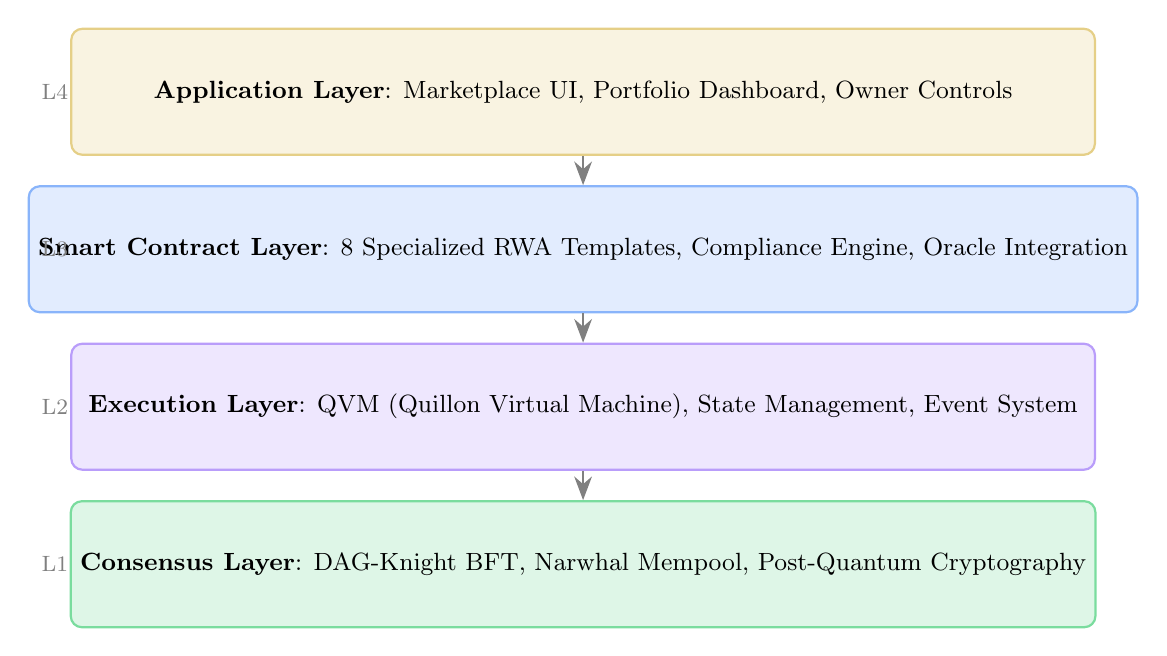
\begin{tikzpicture}[
  layer/.style={draw, thick, rounded corners=4pt, minimum width=13cm, minimum height=1.6cm, font=\small},
  label/.style={font=\footnotesize\color{gray}, anchor=west}
]
  % Layer 4: Application
  \node[layer, fill=qnkgold!15, draw=qnkgold!60] (app) at (0,6)
    {\textbf{Application Layer}: Marketplace UI, Portfolio Dashboard, Owner Controls};

  % Layer 3: Smart Contract
  \node[layer, fill=qnkblue!15, draw=qnkblue!60] (sc) at (0,4)
    {\textbf{Smart Contract Layer}: 8 Specialized RWA Templates, Compliance Engine, Oracle Integration};

  % Layer 2: Execution
  \node[layer, fill=qnkpurple!15, draw=qnkpurple!60] (exec) at (0,2)
    {\textbf{Execution Layer}: QVM (Quillon Virtual Machine), State Management, Event System};

  % Layer 1: Consensus
  \node[layer, fill=qnkgreen!15, draw=qnkgreen!60] (cons) at (0,0)
    {\textbf{Consensus Layer}: DAG-Knight BFT, Narwhal Mempool, Post-Quantum Cryptography};

  % Labels
  \node[label] at (-7,6) {L4};
  \node[label] at (-7,4) {L3};
  \node[label] at (-7,2) {L2};
  \node[label] at (-7,0) {L1};

  % Arrows
  \draw[-{Stealth[length=3mm]}, thick, gray] (app.south) -- (sc.north);
  \draw[-{Stealth[length=3mm]}, thick, gray] (sc.south) -- (exec.north);
  \draw[-{Stealth[length=3mm]}, thick, gray] (exec.south) -- (cons.north);
\end{tikzpicture}
\caption{Q-NarwhalKnight RWA System Architecture}
\label{fig:architecture}
\end{figure}

\subsection{DAG-Knight Consensus}

The consensus layer employs DAG-Knight, a Directed Acyclic Graph-based Byzantine Fault Tolerant protocol that achieves:

\begin{itemize}
  \item \textbf{Sub-3-second finality}: Transactions are confirmed in under 2.9 seconds, enabling real-time settlement of RWA trades.
  \item \textbf{48,000+ TPS}: High throughput supports large-scale asset marketplaces with thousands of concurrent trades.
  \item \textbf{Zero-message-complexity BFT}: Consensus is derived from the DAG structure itself, eliminating the $O(n^2)$ message complexity of PBFT-style protocols.
  \item \textbf{Asynchronous safety}: The protocol remains safe under arbitrary network delays, critical for cross-jurisdictional RWA settlement.
\end{itemize}

\begin{definition}[DAG-Knight Ordering]
Given a DAG $G = (V, E)$ where vertices represent blocks and edges represent references, the DAG-Knight ordering function $\mathcal{O}: V \rightarrow \mathbb{N}$ assigns a total order to all vertices such that:
\begin{equation}
\forall (u, v) \in E: \mathcal{O}(u) < \mathcal{O}(v) \implies u \text{ is confirmed before } v
\end{equation}
with the property that once $\mathcal{O}(v)$ is assigned, it is immutable under any future DAG extension consistent with $f < n/3$ Byzantine validators.
\end{definition}

\subsection{Quillon Virtual Machine (QVM)}

The QVM executes RWA smart contracts within a sandboxed environment:

\begin{itemize}
  \item \textbf{Deterministic execution}: All contract operations produce identical results across all validators.
  \item \textbf{Gas metering}: Dynamic gas pricing targets \$0.10--\$0.50 USD equivalent per deployment, with multipliers based on contract complexity (Table~\ref{tab:gas-multipliers}).
  \item \textbf{State snapshots}: Contract state is captured in Merkle-Patricia tries, enabling efficient proof generation for compliance audits.
  \item \textbf{Event emission}: Contracts emit typed events (SSE) for real-time dashboard updates, including price changes, balance updates, and compliance status.
\end{itemize}

\begin{table}[H]
\centering
\caption{Gas Fee Multipliers by Contract Template}
\label{tab:gas-multipliers}
\begin{tabular}{@{}lccl@{}}
\toprule
\textbf{Template} & \textbf{Multiplier} & \textbf{Est. Cost (USD)} & \textbf{Complexity} \\
\midrule
Secure Token       & 1.0$\times$ & \$0.10 & Basic transfer + balance \\
Advanced Token     & 2.0$\times$ & \$0.20 & Mint, burn, stake, govern \\
Generic RWA        & 3.0$\times$ & \$0.30 & Asset backing + compliance \\
Carbon Credits     & 3.0$\times$ & \$0.30 & Retirement + verification \\
Fixed Income       & 3.5$\times$ & \$0.35 & Coupon payments + maturity \\
Commodities        & 3.5$\times$ & \$0.35 & Storage proof + delivery \\
Art \& Collectibles & 3.5$\times$ & \$0.35 & Provenance + appraisal \\
IP \& Royalties    & 3.5$\times$ & \$0.35 & Revenue sharing + licenses \\
Physical Goods     & 3.5$\times$ & \$0.35 & Supply chain + redemption \\
Real Estate        & 4.0$\times$ & \$0.40 & Yields + fractional ownership \\
Equity \& Shares   & 4.0$\times$ & \$0.45 & Voting + dividends + vesting \\
Private DEX        & 5.0$\times$ & \$0.50 & ZK-SNARK AMM \\
\bottomrule
\end{tabular}
\end{table}

\subsection{Oracle Integration}

RWA tokens require reliable external price feeds and asset verification. Q-NarwhalKnight implements a multi-source oracle system:

\begin{enumerate}
  \item \textbf{Price Oracles}: On-chain price history maintained per token, updated via DEX swap events and external feed submissions.
  \item \textbf{Verification Oracles}: Third-party attestation of asset backing (e.g., property appraisals, commodity storage proofs, carbon credit verification bodies).
  \item \textbf{Compliance Oracles}: KYC/AML status feeds from regulated identity providers, enabling real-time transfer restriction enforcement.
\end{enumerate}

% ═══════════════════════════════════════════════════════════════════════════════
% SECTION 3: SPECIALIZED ASSET CLASSES
% ═══════════════════════════════════════════════════════════════════════════════
\section{Specialized Asset Classes}
\label{sec:asset-classes}

Q-NarwhalKnight provides eight specialized RWA smart contract templates, each designed with domain-specific logic that goes far beyond generic token standards.

\subsection{Real Estate Tokenization}
\label{subsec:real-estate}

\begin{keyinsight}[Real Estate Token Features]
\textbf{Contract Type:} \texttt{real\_estate\_token}\\
\textbf{Key Parameters:} Property type (residential, commercial, industrial, land, mixed-use), location, total valuation (USD), property area (sqft), rental yield (\%), occupancy rate (\%)\\
\textbf{Compliance:} KYC/AML required, accredited investor option, transfer restrictions, dividend distribution\\
\textbf{Gas Cost:} $\sim$\$0.40 USD (4.0$\times$ multiplier)
\end{keyinsight}

Real estate represents the largest single asset class globally at approximately \$326 trillion. Tokenization enables fractional ownership of properties that would otherwise require six- to nine-figure investments.

\subsubsection{Smart Contract Architecture}

The real estate smart contract manages the complete property lifecycle:

\begin{enumerate}[label=\textbf{(\alph*)}]
  \item \textbf{Fractional Ownership}: The property valuation is divided into $N$ shares, each represented as a fungible token. Share count is configurable at deployment via \texttt{total\_shares}.

  \item \textbf{Rental Yield Distribution}: When \texttt{dividend\_enabled} is true, rental income is automatically distributed to token holders proportional to their holdings. Distribution is triggered by the property manager via the \texttt{distribute\_revenue} action.

  \item \textbf{Property Valuation Updates}: The owner can update the on-chain property valuation via \texttt{update\_property\_valuation}, which recalculates the per-share price and emits a price update event.

  \item \textbf{Occupancy Tracking}: Real-time occupancy rate and rental yield metrics are maintained on-chain, enabling investors to assess property performance without relying on off-chain reports.
\end{enumerate}

\begin{figure}[H]
\centering
\begin{tikzpicture}[
  box/.style={draw, thick, rounded corners=3pt, minimum width=3.5cm, minimum height=1.2cm, font=\small, align=center},
  arr/.style={-{Stealth[length=2.5mm]}, thick}
]
  \node[box, fill=qnkgold!15, draw=qnkgold!60] (deploy) at (0,0) {Deploy\\Contract};
  \node[box, fill=qnkblue!15, draw=qnkblue!60] (invest) at (5,0) {Investor\\Purchases Shares};
  \node[box, fill=qnkgreen!15, draw=qnkgreen!60] (rental) at (10,0) {Rental Income\\Received};
  \node[box, fill=qnkpurple!15, draw=qnkpurple!60] (dist) at (5,-2.5) {Dividend\\Distribution};
  \node[box, fill=qnkorange!15, draw=qnkorange!60] (update) at (0,-2.5) {Valuation\\Update};

  \draw[arr] (deploy) -- (invest);
  \draw[arr] (invest) -- (rental);
  \draw[arr] (rental) -- (dist);
  \draw[arr] (dist) -- (update);
  \draw[arr, dashed] (update) -- (deploy) node[midpoint, above, font=\footnotesize] {cycle};
\end{tikzpicture}
\caption{Real Estate Token Lifecycle}
\label{fig:real-estate-lifecycle}
\end{figure}

\subsubsection{Owner Controls}

Post-deployment, the property manager has access to:
\begin{itemize}
  \item \textbf{Update Property Valuation}: Input new appraisal value in USD, automatically recalculates per-share pricing.
  \item \textbf{Update Occupancy \& Yield}: Modify current occupancy rate and rental yield percentage.
  \item \textbf{Distribute Revenue}: Trigger proportional rental income distribution to all token holders.
  \item \textbf{Manage Compliance}: Update KYC whitelist, enable/disable transfer restrictions.
  \item \textbf{Insurance Management}: Update insurance policy status and coverage details.
\end{itemize}

\subsection{Equity \& Shares Tokenization}
\label{subsec:equity}

\begin{keyinsight}[Equity Token Features]
\textbf{Contract Type:} \texttt{equity\_token}\\
\textbf{Key Parameters:} Share class (common, preferred, restricted), company name, dividend schedule (quarterly, semi-annual, annual), vesting period (months), lock-up period (months)\\
\textbf{Governance:} Board seats per share, voting rights, shareholder proposals\\
\textbf{Gas Cost:} $\sim$\$0.45 USD (4.0$\times$ multiplier)
\end{keyinsight}

Equity tokenization transforms private company shares into tradable digital instruments, dramatically reducing the friction of private market transactions.

\subsubsection{Governance Mechanisms}

\begin{itemize}
  \item \textbf{Shareholder Voting}: When \texttt{voting\_rights} is enabled, token holders can create and vote on proposals. Voting power is proportional to share holdings.
  \item \textbf{Vesting Schedules}: Shares vest linearly over the configured \texttt{vesting\_period\_months}, with a cliff at \texttt{lockup\_period\_months}.
  \item \textbf{Dividend Distribution}: Configurable dividend schedules (quarterly, semi-annual, annual) with automatic proportional distribution.
  \item \textbf{Share Class Differentiation}: Common shares carry voting rights; preferred shares receive priority dividends; restricted stock is subject to vesting.
\end{itemize}

\subsection{Fixed Income \& Bonds}
\label{subsec:fixed-income}

\begin{keyinsight}[Fixed Income Token Features]
\textbf{Contract Type:} \texttt{fixed\_income\_token}\\
\textbf{Key Parameters:} Instrument type (corporate bond, treasury note, municipal bond, convertible note), face value (USD), coupon rate (\%), maturity date, payment frequency, credit rating (AAA--B)\\
\textbf{Special Features:} Callable, convertible to equity\\
\textbf{Gas Cost:} $\sim$\$0.35 USD (3.5$\times$ multiplier)
\end{keyinsight}

\subsubsection{Bond Lifecycle Management}

The fixed income smart contract automates the complete bond lifecycle:

\begin{enumerate}
  \item \textbf{Coupon Payments}: Periodic interest payments at the configured \texttt{payment\_frequency} (monthly, quarterly, semi-annual, or annual) at the specified \texttt{coupon\_rate\_percent}.

  \item \textbf{Maturity Handling}: At \texttt{maturity\_date}, the contract automatically triggers principal repayment to all token holders.

  \item \textbf{Call Provisions}: When \texttt{callable} is true, the issuer can redeem the bond before maturity at a specified call price.

  \item \textbf{Conversion}: When \texttt{convertible} is true, bondholders can convert their debt instruments to equity tokens at a predetermined conversion ratio.

  \item \textbf{Credit Rating}: The \texttt{credit\_rating} (AAA through B) is stored on-chain and can be updated by the issuer following rating agency reviews.
\end{enumerate}

\subsection{Commodity Tokenization}
\label{subsec:commodities}

\begin{keyinsight}[Commodity Token Features]
\textbf{Contract Type:} \texttt{commodity\_token}\\
\textbf{Key Parameters:} Commodity type (precious metal, energy, agriculture, industrial metal), unit of measurement (troy oz, kg, barrel, bushel, MWh), quantity per token, storage provider, storage location\\
\textbf{Special Features:} Physical delivery option, insurance, spot price oracle\\
\textbf{Gas Cost:} $\sim$\$0.35 USD (3.5$\times$ multiplier)
\end{keyinsight}

\subsubsection{Storage Proof and Delivery}

\begin{itemize}
  \item \textbf{Storage Proof}: The contract maintains verifiable proof that the underlying commodity exists in the specified storage facility (e.g., Brinks vault in London, Loomis warehouse in Zurich).
  \item \textbf{Physical Delivery}: When \texttt{delivery\_option} is enabled, token holders can redeem tokens for physical delivery of the underlying commodity.
  \item \textbf{Spot Price Oracle}: Integration with external price feeds (e.g., XAU/USD for gold) enables real-time mark-to-market pricing.
  \item \textbf{Insurance}: When \texttt{insurance\_enabled} is true, the stored commodity is insured against loss, theft, or damage.
\end{itemize}

\subsection{Carbon Credit Tokenization}
\label{subsec:carbon}

\begin{keyinsight}[Carbon Credit Token Features]
\textbf{Contract Type:} \texttt{carbon\_credit\_token}\\
\textbf{Key Parameters:} Credit standard (Verra VCS, Gold Standard, ACR, CAR), project type (reforestation, renewable energy, methane capture, direct air capture, ocean conservation), vintage year, total credits (tonnes CO$_2$), verification body, project location\\
\textbf{Special Features:} Credit retirement, offset tracking, offset certificates\\
\textbf{Gas Cost:} $\sim$\$0.30 USD (3.0$\times$ multiplier)
\end{keyinsight}

\subsubsection{Environmental Impact Tracking}

Carbon credit tokenization requires special handling to prevent double-counting and ensure environmental integrity:

\begin{enumerate}
  \item \textbf{Credit Retirement}: When \texttt{retirement\_enabled} is true, token holders can permanently retire credits, removing them from circulation. Retired credits are recorded immutably on-chain with the retiring entity's identity.

  \item \textbf{Offset Certificates}: When \texttt{offset\_tracking} is true, the contract issues verifiable offset certificates for each retirement event, suitable for corporate ESG reporting.

  \item \textbf{Verification Status}: The contract maintains the verification status from the accredited verification body (e.g., SCS Global Services), which can be updated by the project owner.

  \item \textbf{Vintage Tracking}: Each credit token carries its vintage year, ensuring temporal accuracy in carbon accounting.
\end{enumerate}

\begin{figure}[H]
\centering
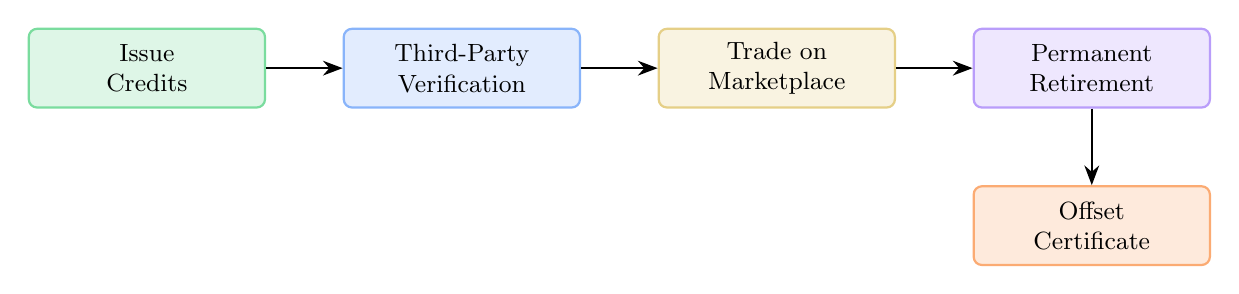
\begin{tikzpicture}[
  box/.style={draw, thick, rounded corners=3pt, minimum width=3cm, minimum height=1cm, font=\small, align=center},
  arr/.style={-{Stealth[length=2.5mm]}, thick}
]
  \node[box, fill=qnkgreen!15, draw=qnkgreen!60] (issue) at (0,0) {Issue\\Credits};
  \node[box, fill=qnkblue!15, draw=qnkblue!60] (verify) at (4,0) {Third-Party\\Verification};
  \node[box, fill=qnkgold!15, draw=qnkgold!60] (trade) at (8,0) {Trade on\\Marketplace};
  \node[box, fill=qnkpurple!15, draw=qnkpurple!60] (retire) at (12,0) {Permanent\\Retirement};
  \node[box, fill=qnkorange!15, draw=qnkorange!60] (cert) at (12,-2) {Offset\\Certificate};

  \draw[arr] (issue) -- (verify);
  \draw[arr] (verify) -- (trade);
  \draw[arr] (trade) -- (retire);
  \draw[arr] (retire) -- (cert);
\end{tikzpicture}
\caption{Carbon Credit Token Lifecycle}
\label{fig:carbon-lifecycle}
\end{figure}

\subsection{Art \& Collectibles Tokenization}
\label{subsec:art}

\begin{keyinsight}[Art \& Collectibles Token Features]
\textbf{Contract Type:} \texttt{art\_collectible\_token}\\
\textbf{Key Parameters:} Item type (painting, sculpture, digital art, photography, rare collectible, wine \& spirits), artist/creator, creation year, appraisal value (USD), total fractions, physical custody (owner, vault, museum, gallery)\\
\textbf{Special Features:} Provenance verification, insurance\\
\textbf{Gas Cost:} $\sim$\$0.35 USD (3.5$\times$ multiplier)
\end{keyinsight}

\subsubsection{Provenance and Authentication}

The art tokenization contract maintains an immutable provenance chain:

\begin{itemize}
  \item \textbf{Provenance Chain}: Every ownership transfer, exhibition, and conservation event is recorded on-chain, creating an unbroken chain of custody from creation to present.
  \item \textbf{Appraisal History}: Professional appraisals are timestamped and stored, enabling investors to track value appreciation over time.
  \item \textbf{Custody Tracking}: The physical location (owner, secure vault, museum, gallery) is maintained on-chain with update capabilities for the asset manager.
  \item \textbf{Fractional Ownership}: High-value artworks are divided into fractions, enabling retail investors to own portions of blue-chip art.
\end{itemize}

\subsection{IP \& Royalty Tokenization}
\label{subsec:ip}

\begin{keyinsight}[IP \& Royalty Token Features]
\textbf{Contract Type:} \texttt{ip\_revenue\_token}\\
\textbf{Key Parameters:} IP type (patent, copyright, trademark, music royalty, film royalty, software license), jurisdiction, registration number, revenue share (\%), expiry date, distribution frequency, minimum guarantee (USD)\\
\textbf{Special Features:} Sublicensing, royalty distribution\\
\textbf{Gas Cost:} $\sim$\$0.35 USD (3.5$\times$ multiplier)
\end{keyinsight}

\subsubsection{Revenue Stream Tokenization}

IP tokenization converts future revenue streams into tradable tokens:

\begin{enumerate}
  \item \textbf{Revenue Sharing}: Token holders receive a proportional share of the IP revenue at the configured \texttt{revenue\_share\_percent}.
  \item \textbf{Automatic Distribution}: Revenue is distributed at the specified \texttt{distribution\_frequency} (monthly, quarterly, or annually).
  \item \textbf{Minimum Guarantee}: The \texttt{minimum\_guarantee\_usd} ensures token holders receive a minimum return regardless of actual IP revenue.
  \item \textbf{Sublicensing}: When \texttt{sublicensing\_allowed} is true, the IP can be sublicensed to third parties, with sublicensing revenue flowing to token holders.
\end{enumerate}

\subsection{Physical Goods Tokenization}
\label{subsec:physical-goods}

\begin{keyinsight}[Physical Goods Token Features]
\textbf{Contract Type:} \texttt{physical\_goods\_token}\\
\textbf{Key Parameters:} Product category (luxury goods, electronics, automotive, jewelry, watches), manufacturer/brand, warehouse location\\
\textbf{Special Features:} Serial number tracking, supply chain verification, physical redemption, shipping, insurance\\
\textbf{Gas Cost:} $\sim$\$0.35 USD (3.5$\times$ multiplier)
\end{keyinsight}

\subsubsection{Supply Chain Integration}

\begin{itemize}
  \item \textbf{Serial Number Tracking}: Each physical item is tracked by serial number, preventing counterfeiting and enabling provenance verification.
  \item \textbf{Supply Chain Verification}: Full supply chain provenance from manufacturer to warehouse is recorded on-chain.
  \item \textbf{Physical Redemption}: Token holders can redeem tokens for the physical item, triggering a logistics workflow.
  \item \textbf{Inventory Management}: The contract tracks warehouse inventory levels, ensuring tokens are always backed by physical goods.
\end{itemize}

% ═══════════════════════════════════════════════════════════════════════════════
% SECTION 4: COMPLIANCE FRAMEWORK
% ═══════════════════════════════════════════════════════════════════════════════
\section{Compliance Framework}
\label{sec:compliance}

\subsection{Regulatory Landscape}

RWA tokenization operates at the intersection of securities law, banking regulation, and digital asset legislation. Q-NarwhalKnight's compliance framework addresses:

\begin{compliancebox}[Regulatory Coverage]
\begin{tabularx}{\textwidth}{lX}
\textbf{Regulation} & \textbf{Implementation} \\
\midrule
SEC Regulation D (506b/c) & Accredited investor gates via \texttt{accredited\_only} flag \\
SEC Regulation S & Jurisdictional transfer restrictions via whitelist \\
KYC/AML (BSA, 6AMLD) & Identity verification gate via \texttt{kyc\_required} flag \\
MiCA (EU) & Asset classification and transparency requirements \\
FATF Travel Rule & Transfer metadata propagation between VASPs \\
Reg A+ / Reg CF & Configurable investment limits and disclosure requirements \\
\end{tabularx}
\end{compliancebox}

\subsection{On-Chain Compliance Primitives}

\subsubsection{KYC/AML Verification}

When \texttt{kyc\_required} is enabled on an RWA contract, every transfer is checked against a KYC whitelist:

\begin{algorithm}[H]
\caption{KYC-Gated Transfer}
\label{alg:kyc-transfer}
\begin{algorithmic}[1]
\Procedure{Transfer}{$\textit{from}, \textit{to}, \textit{amount}$}
  \If{contract.kyc\_required}
    \If{$\neg$ \Call{IsKYCVerified}{$\textit{from}$} $\lor$ $\neg$ \Call{IsKYCVerified}{$\textit{to}$}}
      \State \Return \textsc{Error}(``KYC verification required'')
    \EndIf
  \EndIf
  \If{contract.accredited\_only}
    \If{$\neg$ \Call{IsAccredited}{$\textit{to}$}}
      \State \Return \textsc{Error}(``Accredited investors only'')
    \EndIf
  \EndIf
  \If{contract.transfer\_restrictions}
    \If{$\neg$ \Call{IsWhitelisted}{$\textit{to}$}}
      \State \Return \textsc{Error}(``Address not on transfer whitelist'')
    \EndIf
  \EndIf
  \State \Call{ExecuteTransfer}{$\textit{from}, \textit{to}, \textit{amount}$}
\EndProcedure
\end{algorithmic}
\end{algorithm}

\subsubsection{Transfer Restriction Whitelist}

The contract owner maintains a whitelist of addresses permitted to receive tokens. This enables:

\begin{itemize}
  \item \textbf{Jurisdictional Compliance}: Restrict transfers to addresses in permitted jurisdictions.
  \item \textbf{Investor Qualification}: Ensure all holders meet ongoing qualification requirements.
  \item \textbf{Lock-Up Enforcement}: Prevent transfers during lock-up periods.
  \item \textbf{Sanctions Screening}: Block transfers to sanctioned addresses.
\end{itemize}

\subsection{Compliance Audit Trail}

Every compliance-relevant event is immutably recorded on the DAG:

\begin{itemize}
  \item KYC verification status changes
  \item Whitelist additions and removals
  \item Transfer restriction enforcement events
  \item Dividend distributions with recipient verification
  \item Ownership concentration alerts
\end{itemize}

This creates a complete audit trail suitable for regulatory examination, accessible via the contract's event history interface.

% ═══════════════════════════════════════════════════════════════════════════════
% SECTION 5: POST-QUANTUM SECURITY
% ═══════════════════════════════════════════════════════════════════════════════
\section{Post-Quantum Security}
\label{sec:pq-security}

\subsection{The Quantum Threat to RWA Tokens}

\begin{securitybox}[Critical: Why RWA Tokens Are Uniquely Vulnerable]
Unlike speculative cryptocurrencies, RWA tokens represent claims on real-world assets with multi-decade lifespans. A property token issued today must remain secure for the 30+ year life of the underlying real estate. Quantum computers capable of breaking ECDSA (estimated 2030--2040) would allow an adversary to:
\begin{enumerate}
  \item Forge transfer signatures, stealing tokenized property
  \item Manipulate governance votes to seize corporate control
  \item Break compliance mechanisms, enabling unauthorized transfers
  \item Retroactively forge the entire provenance chain
\end{enumerate}
\end{securitybox}

\subsection{Cryptographic Primitives}

Q-NarwhalKnight employs NIST PQC standard algorithms:

\begin{table}[H]
\centering
\caption{Post-Quantum Cryptographic Primitives}
\label{tab:pq-primitives}
\begin{tabular}{@{}lllr@{}}
\toprule
\textbf{Primitive} & \textbf{Algorithm} & \textbf{NIST Level} & \textbf{Security (bits)} \\
\midrule
Digital Signatures & Dilithium5 (ML-DSA-87) & Level 5 & 256 \\
Key Encapsulation  & Kyber1024 (ML-KEM-1024) & Level 5 & 256 \\
Hash Functions     & SHA-3 (Keccak-256) & --- & 256 \\
VDF                & Genus-2 Isogeny VDF & --- & 128+ \\
\bottomrule
\end{tabular}
\end{table}

\subsection{Crypto-Agile Framework}

The system implements a height-gated upgrade mechanism for cryptographic transitions:

\begin{theorem}[Backward-Compatible Cryptographic Upgrades]
Let $H_{\text{activate}}$ be the activation height for a new cryptographic primitive. For all blocks $B$ with height $h(B)$:
\begin{equation}
\text{Verify}(B) =
\begin{cases}
\text{Verify}_{\text{old}}(B) & \text{if } h(B) < H_{\text{activate}} \\
\text{Verify}_{\text{new}}(B) & \text{if } h(B) \geq H_{\text{activate}}
\end{cases}
\end{equation}
This ensures historical blocks always validate under their original rules, while new blocks use upgraded cryptography.
\end{theorem}

This is critical for RWA tokens where the provenance chain must remain verifiable indefinitely---old property transfers verified with Ed25519 remain valid while new transfers use Dilithium5.

\subsection{Quantum-Resistant Asset Security Properties}

\begin{property}[Long-Term Asset Security]
For an RWA token $T$ representing asset $A$ with lifetime $L$ years, the probability of a successful cryptographic attack is:
\begin{equation}
P_{\text{attack}} \leq \frac{L \cdot 2^{40}}{2^{256}} = L \cdot 2^{-216} \approx 0
\end{equation}
for Dilithium5 (256-bit security), even under aggressive quantum computing advancement assumptions.
\end{property}

% ═══════════════════════════════════════════════════════════════════════════════
% SECTION 6: RWA MARKETPLACE
% ═══════════════════════════════════════════════════════════════════════════════
\section{RWA Marketplace}
\label{sec:marketplace}

\subsection{Marketplace Architecture}

The RWA Marketplace provides a unified interface for discovering, analyzing, and investing in tokenized real-world assets. The design follows a premium aesthetic inspired by luxury automotive brands, emphasizing trust, sophistication, and clarity.

\subsubsection{Discovery and Filtering}

\begin{itemize}
  \item \textbf{Category Filtering}: Assets are organized by the eight specialized categories, with an ``All Assets'' view for cross-category discovery.
  \item \textbf{Search}: Full-text search across asset names, symbols, descriptions, and deployment parameters.
  \item \textbf{Sorting}: By total value, price per share, deployment date, or name.
  \item \textbf{View Modes}: Grid view for visual browsing, list view for data-dense comparison.
\end{itemize}

\subsubsection{Asset Detail Cards}

Each asset listing displays:
\begin{itemize}
  \item Total asset value (USD)
  \item Available shares and price per share
  \item Compliance badges (KYC Required, Dividends Enabled, Verified Asset)
  \item Feature flags specific to the asset class
  \item Contract address with copy functionality
\end{itemize}

\subsubsection{Investment Flow}

\begin{enumerate}
  \item Investor selects asset from marketplace
  \item Detail modal displays comprehensive asset information
  \item Investor enters desired number of shares
  \item Estimated cost is calculated in real-time
  \item Investment transaction is submitted to the DAG
  \item Shares appear in investor's portfolio upon confirmation ($<$3 seconds)
\end{enumerate}

\subsection{Portfolio Management}

The Portfolio tab provides investors with:
\begin{itemize}
  \item Total portfolio value across all RWA holdings
  \item Per-asset breakdown with current value, cost basis, and unrealized P\&L
  \item Dividend/coupon payment history
  \item Compliance status for each holding
\end{itemize}

% ═══════════════════════════════════════════════════════════════════════════════
% SECTION 7: POST-DEPLOYMENT OWNER CONTROLS
% ═══════════════════════════════════════════════════════════════════════════════
\section{Post-Deployment Owner Controls}
\label{sec:owner-controls}

\subsection{Design Philosophy}

Unlike traditional tokens where smart contracts are immutable black boxes after deployment, Q-NarwhalKnight RWA tokens provide comprehensive post-deployment management interfaces. This reflects the reality that real-world assets require ongoing management---properties need valuation updates, bonds require coupon payments, carbon credits need verification renewals.

\subsection{Control Categories}

Each RWA type exposes a unique set of controls organized into functional categories:

\begin{table}[H]
\centering
\caption{Post-Deployment Owner Controls by Asset Class}
\label{tab:owner-controls}
\footnotesize
\begin{tabularx}{\textwidth}{@{}l|X@{}}
\toprule
\textbf{Asset Class} & \textbf{Available Controls} \\
\midrule
\textbf{Real Estate} & Update valuation, update occupancy/yield, distribute rental revenue, manage KYC whitelist, update insurance \\
\midrule
\textbf{Equity} & Create shareholder proposals, initiate voting, distribute dividends, manage vesting schedules, update board governance \\
\midrule
\textbf{Fixed Income} & Issue coupon payments, call bonds, enable conversion to equity, update credit rating \\
\midrule
\textbf{Commodities} & Update storage proof, process delivery requests, update spot price, manage insurance, update inventory \\
\midrule
\textbf{Carbon Credits} & Update verification status, issue offset certificates, retire credits, update project metrics \\
\midrule
\textbf{Art \& Collectibles} & Update appraisal value, update custody location, verify provenance, manage insurance \\
\midrule
\textbf{IP \& Royalties} & Distribute royalties, manage sublicenses, update revenue projections, renew IP registration \\
\midrule
\textbf{Physical Goods} & Process redemption requests, update inventory, verify supply chain, manage shipping, update insurance \\
\bottomrule
\end{tabularx}
\end{table}

\subsection{Interaction Protocol}

All owner control actions follow a standardized interaction protocol:

\begin{algorithm}[H]
\caption{Contract Interaction Protocol}
\label{alg:interaction}
\begin{algorithmic}[1]
\Procedure{ContractAction}{$\textit{contract}, \textit{action}, \textit{params}$}
  \State $\textit{tx} \gets$ \Call{BuildTransaction}{contract.address, action, params}
  \State $\textit{sig} \gets$ \Call{Sign}{tx, owner.private\_key} \Comment{Dilithium5 signature}
  \State \Call{Submit}{tx, sig}
  \State $\textit{result} \gets$ \Call{AwaitConfirmation}{tx.hash} \Comment{$<$3 second finality}
  \State \Call{EmitSSE}{contract.address, action, result} \Comment{Real-time UI update}
  \State \Return result
\EndProcedure
\end{algorithmic}
\end{algorithm}

The UI provides inline feedback for each action: loading spinner during submission, success/error messages upon completion, with automatic status clearing after 5 seconds.

% ═══════════════════════════════════════════════════════════════════════════════
% SECTION 8: ECONOMIC MODEL
% ═══════════════════════════════════════════════════════════════════════════════
\section{Economic Model}
\label{sec:economics}

\subsection{Fee Structure}

The Q-NarwhalKnight RWA platform uses a dynamic fee model targeting USD-equivalent costs:

\begin{equation}
\text{Fee}_{\text{QUG}} = \frac{\text{BaseCost}_{\text{USD}} \times \text{Multiplier}_{\text{template}}}{\text{Price}_{\text{QUG/USD}}}
\end{equation}

where $\text{BaseCost}_{\text{USD}} = \$0.10$ and $\text{Multiplier}_{\text{template}}$ ranges from 1.0$\times$ (simple token) to 5.0$\times$ (Private DEX with ZK-SNARKs).

This ensures deployment costs remain stable in USD terms regardless of QUG token price volatility, addressing a critical pain point of Ethereum-based tokenization where gas fees can spike to hundreds of dollars.

\subsection{Revenue Distribution Mechanics}

For dividend-bearing tokens (real estate, equity, bonds, IP royalties):

\begin{equation}
\text{Dividend}_i = \text{TotalRevenue} \times \frac{\text{Balance}_i}{\text{TotalSupply}}
\end{equation}

where $\text{Dividend}_i$ is the payout to holder $i$, distributed atomically in a single transaction to prevent front-running.

\subsection{DEX Integration}

RWA tokens are tradable on the integrated Q-NarwhalKnight DEX:

\begin{itemize}
  \item \textbf{AMM Liquidity Pools}: Automated Market Maker pools for RWA/QUG trading pairs.
  \item \textbf{Cross-Decimal Support}: The AMM correctly handles tokens with different decimal precisions (8 vs 24 decimals).
  \item \textbf{Compliance-Aware Trading}: DEX enforces transfer restrictions---only whitelisted addresses can receive compliance-restricted tokens via swaps.
  \item \textbf{Price Oracle Updates}: Every DEX swap updates the on-chain price oracle, ensuring real-time valuation accuracy.
\end{itemize}

% ═══════════════════════════════════════════════════════════════════════════════
% SECTION 9: RISK ANALYSIS
% ═══════════════════════════════════════════════════════════════════════════════
\section{Risk Analysis}
\label{sec:risk}

\subsection{Smart Contract Risk}

\begin{table}[H]
\centering
\caption{Risk Matrix for RWA Smart Contracts}
\label{tab:risk-matrix}
\begin{tabular}{@{}llll@{}}
\toprule
\textbf{Risk} & \textbf{Likelihood} & \textbf{Impact} & \textbf{Mitigation} \\
\midrule
Logic bugs in contracts & Medium & High & 4,000+ automated tests \\
Oracle manipulation & Low & High & Multi-source oracle aggregation \\
Key compromise & Low & Critical & Dilithium5 PQ signatures \\
Regulatory change & Medium & Medium & Height-gated upgrade mechanism \\
Liquidity crisis & Medium & Medium & AMM with minimum liquidity \\
Custodial failure & Low & High & Multi-custodian support \\
\bottomrule
\end{tabular}
\end{table}

\subsection{Regulatory Risk}

The height-gated upgrade mechanism (Section~\ref{sec:pq-security}) enables compliance rule updates without hard forks:

\begin{itemize}
  \item New regulatory requirements can be activated at a future block height.
  \item Existing tokens continue operating under their deployment-time rules until the upgrade height.
  \item Emergency compliance changes can be deployed with a short activation horizon.
\end{itemize}

\subsection{Custody and Counterparty Risk}

RWA tokens are only as good as their real-world backing. Q-NarwhalKnight mitigates custody risk through:

\begin{enumerate}
  \item \textbf{Verification Oracles}: Third-party attestation of asset existence and condition.
  \item \textbf{Insurance Requirements}: Optional but recommended insurance for physical assets.
  \item \textbf{Audit Trails}: Complete on-chain record of all custody changes and verifications.
  \item \textbf{Multi-Custodian Support}: Assets can be distributed across multiple custodians.
\end{enumerate}

% ═══════════════════════════════════════════════════════════════════════════════
% SECTION 10: COMPARISON WITH EXISTING PLATFORMS
% ═══════════════════════════════════════════════════════════════════════════════
\section{Comparison with Existing Platforms}
\label{sec:comparison}

\begin{table}[H]
\centering
\caption{Platform Comparison Matrix}
\label{tab:comparison}
\footnotesize
\begin{tabularx}{\textwidth}{@{}l|c|c|c|c|X@{}}
\toprule
\textbf{Feature} & \textbf{QNK} & \textbf{ETH} & \textbf{Polygon} & \textbf{Stellar} & \textbf{Notes} \\
\midrule
Post-Quantum Security & \checkmark & $\times$ & $\times$ & $\times$ & QNK: Dilithium5 Level 5 \\
Specialized RWA Templates & 8 & 0 & 0 & 0 & Others use generic ERC-20/1400 \\
Sub-3s Finality & \checkmark & $\times$ & $\sim$ & \checkmark & ETH: 12 min (finality gadget) \\
Embedded Compliance & \checkmark & $\times$ & $\times$ & $\sim$ & QNK: First-class primitives \\
Owner Controls UI & \checkmark & $\times$ & $\times$ & $\times$ & QNK: In-wallet management \\
Deployment Cost & \$0.40 & \$50+ & \$0.10 & \$0.01 & QNK: Stable USD-targeted \\
Throughput (TPS) & 48K+ & 15 & 7K & 1K & QNK: DAG-Knight parallel \\
Crypto-Agile Upgrades & \checkmark & $\times$ & $\times$ & $\times$ & Height-gated transitions \\
Integrated DEX & \checkmark & DApp & DApp & DEX & QNK: Native AMM \\
Integrated Marketplace & \checkmark & $\times$ & $\times$ & $\times$ & QNK: Built-in RWA store \\
\bottomrule
\end{tabularx}
\end{table}

\subsection{Key Differentiators}

\begin{enumerate}
  \item \textbf{Quantum Security}: Q-NarwhalKnight is the only RWA platform offering NIST Level 5 post-quantum security, critical for assets with multi-decade lifespans.

  \item \textbf{Template Specialization}: Rather than forcing all assets into generic token standards, each asset class gets purpose-built logic (rental yields for real estate, coupon payments for bonds, retirement for carbon credits).

  \item \textbf{Integrated Experience}: Deployment, marketplace listing, trading, and management all occur within the same application, eliminating the need for multiple third-party tools.

  \item \textbf{Dynamic Gas Pricing}: USD-targeted fees prevent the gas price volatility that makes Ethereum-based RWA tokenization impractical for low-value fractions.
\end{enumerate}

% ═══════════════════════════════════════════════════════════════════════════════
% SECTION 11: FUTURE WORK
% ═══════════════════════════════════════════════════════════════════════════════
\section{Future Work}
\label{sec:future}

\subsection{Cross-Chain RWA Bridges}

Future development will enable RWA tokens to be bridged to other blockchains while maintaining compliance controls. The bridge will verify KYC/AML status on the destination chain before releasing tokens.

\subsection{Automated Appraisal Integration}

Integration with professional appraisal APIs will enable automated, oracle-fed property valuations and commodity pricing, reducing reliance on manual owner updates.

\subsection{Legal Entity Wrapping}

Partnership with legal service providers to automatically create SPVs (Special Purpose Vehicles) or LLC wrappers for tokenized assets, providing legal clarity on token holder rights.

\subsection{Insurance Marketplace}

An integrated insurance marketplace where asset owners can purchase coverage from competing insurers, with premium payments and claims management handled on-chain.

\subsection{Secondary Market Order Books}

In addition to AMM-based trading, a central limit order book (CLOB) for RWA tokens will provide better price discovery for less liquid assets.

% ═══════════════════════════════════════════════════════════════════════════════
% SECTION 12: CONCLUSION
% ═══════════════════════════════════════════════════════════════════════════════
\section{Conclusion}
\label{sec:conclusion}

Q-NarwhalKnight's RWA tokenization framework represents a significant advancement in the digitization of real-world assets. By combining post-quantum cryptographic security with specialized smart contract templates, embedded compliance mechanisms, and comprehensive post-deployment management interfaces, the platform addresses the three critical failures of existing tokenization solutions: quantum vulnerability, regulatory inadequacy, and asset class homogeneity.

The eight specialized asset classes---real estate, equity, fixed income, commodities, carbon credits, art \& collectibles, intellectual property, and physical goods---each receive purpose-built smart contract logic that faithfully represents the unique characteristics, compliance requirements, and lifecycle management needs of the underlying assets.

With sub-3-second settlement finality, 48,000+ TPS throughput, and deployment costs under \$0.50, Q-NarwhalKnight makes tokenization economically viable for assets of all sizes, from multi-billion dollar commercial real estate portfolios to individual carbon credit retirements.

As quantum computing advances threaten the cryptographic foundations of existing blockchain platforms, Q-NarwhalKnight's NIST Level 5 post-quantum security ensures that tokenized assets remain secure for their entire multi-decade lifespans. The crypto-agile upgrade mechanism further guarantees that the platform can adopt future cryptographic standards without disrupting existing token holders.

The integration of marketplace discovery, compliance-aware trading, and portfolio management into a single application creates a seamless experience that lowers the barrier to entry for both asset issuers and investors, accelerating the transition from traditional asset markets to tokenized, democratized ownership.

\vspace{1cm}

\begin{center}
\rule{0.5\textwidth}{0.4pt}\\[0.5em]
{\small\itshape ``Tokenization is not about creating digital representations of assets.\\
It is about creating entirely new markets where none existed before.''}\\[0.5em]
\rule{0.5\textwidth}{0.4pt}
\end{center}

% ═══════════════════════════════════════════════════════════════════════════════
% APPENDICES
% ═══════════════════════════════════════════════════════════════════════════════
\appendix

\section{Complete RWA Deployment Parameter Reference}
\label{app:params}

\begin{longtable}{@{}llll@{}}
\caption{Complete Deployment Parameters for All RWA Types} \label{tab:all-params} \\
\toprule
\textbf{Asset Class} & \textbf{Parameter Key} & \textbf{Type} & \textbf{Description} \\
\midrule
\endfirsthead
\toprule
\textbf{Asset Class} & \textbf{Parameter Key} & \textbf{Type} & \textbf{Description} \\
\midrule
\endhead
\bottomrule
\endfoot

\multirow{7}{*}{Real Estate}
  & property\_type & Select & Residential/Commercial/Industrial/Land \\
  & location & Text & Physical address or region \\
  & total\_valuation\_usd & Number & Property value in USD \\
  & property\_area\_sqft & Number & Property size \\
  & rental\_yield\_percent & Number & Annual rental yield \\
  & occupancy\_rate & Number & Current occupancy percentage \\
  & kyc\_required & Boolean & KYC/AML gate \\
\midrule

\multirow{6}{*}{Equity}
  & share\_class & Select & Common/Preferred/Restricted \\
  & company\_name & Text & Issuing company \\
  & dividend\_schedule & Select & Quarterly/Semi-Annual/Annual \\
  & vesting\_period\_months & Number & Vesting duration \\
  & lockup\_period\_months & Number & Lock-up duration \\
  & voting\_rights & Boolean & Governance participation \\
\midrule

\multirow{6}{*}{Fixed Income}
  & instrument\_type & Select & Corporate/Treasury/Municipal/Convertible \\
  & face\_value\_usd & Number & Bond face value \\
  & coupon\_rate\_percent & Number & Interest rate \\
  & maturity\_date & Text & Bond maturity \\
  & credit\_rating & Select & AAA through B \\
  & callable & Boolean & Early redemption allowed \\
\midrule

\multirow{6}{*}{Commodities}
  & commodity\_type & Select & Precious Metal/Energy/Agriculture \\
  & unit\_of\_measurement & Select & Troy Oz/Kg/Barrel/Bushel \\
  & quantity\_per\_token & Number & Physical quantity per token \\
  & storage\_provider & Text & Custodian name \\
  & delivery\_option & Boolean & Physical delivery available \\
  & insurance\_enabled & Boolean & Asset insured \\
\midrule

\multirow{6}{*}{Carbon Credits}
  & credit\_standard & Select & Verra VCS/Gold Standard/ACR/CAR \\
  & project\_type & Select & Reforestation/Renewable/DAC \\
  & vintage\_year & Number & Credit vintage \\
  & total\_credits\_tonnes & Number & Total CO$_2$ tonnes \\
  & retirement\_enabled & Boolean & Permanent retirement \\
  & offset\_tracking & Boolean & Certificate generation \\
\midrule

\multirow{6}{*}{Art \& Collectibles}
  & item\_type & Select & Painting/Sculpture/Digital/Photo \\
  & artist\_creator & Text & Artist or creator \\
  & appraisal\_value\_usd & Number & Current appraisal \\
  & total\_fractions & Number & Fractional shares \\
  & physical\_custody & Select & Owner/Vault/Museum/Gallery \\
  & provenance\_verified & Boolean & Chain of custody verified \\
\midrule

\multirow{6}{*}{IP \& Royalties}
  & ip\_type & Select & Patent/Copyright/Trademark/Royalty \\
  & jurisdiction & Text & Legal jurisdiction \\
  & revenue\_share\_percent & Number & Revenue share for holders \\
  & expiry\_date & Text & IP expiration \\
  & minimum\_guarantee\_usd & Number & Minimum guaranteed return \\
  & sublicensing\_allowed & Boolean & Sublicensing permitted \\
\midrule

\multirow{6}{*}{Physical Goods}
  & product\_category & Select & Luxury/Electronics/Auto/Jewelry \\
  & manufacturer & Text & Brand or manufacturer \\
  & warehouse\_location & Text & Storage facility \\
  & serial\_number\_tracking & Boolean & Individual item tracking \\
  & redemption\_enabled & Boolean & Physical claim available \\
  & shipping\_included & Boolean & Logistics included \\

\end{longtable}

\section{Smart Contract API Reference}
\label{app:api}

\subsection{Deployment Endpoint}

\begin{lstlisting}[style=rustcode, caption={RWA Contract Deployment API}]
POST /api/v1/contracts/deploy
Content-Type: application/json

{
  "template": "real_estate_token",
  "name": "Manhattan Luxury Condo",
  "symbol": "MANLUX",
  "decimals": 8,
  "initial_supply": "1000000",
  "deployment_params": {
    "property_type": "residential",
    "location": "Manhattan, NY",
    "total_valuation_usd": "5000000",
    "rental_yield_percent": "4.5",
    "kyc_required": true,
    "dividend_enabled": true
  }
}
\end{lstlisting}

\subsection{Interaction Endpoint}

\begin{lstlisting}[style=rustcode, caption={RWA Contract Interaction API}]
POST /api/v1/contracts/{address}/interact
Content-Type: application/json

{
  "action": "distribute_revenue",
  "params": {
    "amount": "50000",
    "currency": "USD"
  }
}
\end{lstlisting}

\subsection{Marketplace Query Endpoint}

\begin{lstlisting}[style=rustcode, caption={RWA Marketplace Query API}]
GET /api/v1/contracts/rwa/marketplace?category=real_estate

Response:
{
  "success": true,
  "data": [
    {
      "name": "Manhattan Luxury Condo",
      "symbol": "MANLUX",
      "contract_type": "RealEstateToken",
      "total_value_usd": "5000000",
      "shares_available": "1000000",
      "kyc_required": true,
      "dividend_enabled": true,
      "verified": false,
      "features": {
        "kyc_required": true,
        "dividend_enabled": true,
        "transfer_restrictions": false
      }
    }
  ]
}
\end{lstlisting}

% ─── References ────────────────────────────────────────────────────────────────
\newpage
\begin{thebibliography}{99}

\bibitem{bcg2022}
Boston Consulting Group and ADDX,
``Relevance of On-Chain Asset Tokenization in Crypto Winter,''
BCG Report, 2022.

\bibitem{nist-pqc}
National Institute of Standards and Technology,
``Post-Quantum Cryptography Standardization,''
NIST FIPS 203, 204, 205, August 2024.

\bibitem{dilithium}
L. Ducas, E. Kiltz, T. Lepoint, V. Lyubashevsky, P. Schwabe, G. Seiler, and D. Stehl\'{e},
``CRYSTALS-Dilithium: A Lattice-Based Digital Signature Scheme,''
IACR Transactions on Cryptographic Hardware and Embedded Systems, 2018.

\bibitem{kyber}
R. Avanzi, J. Bos, L. Ducas, E. Kiltz, T. Lepoint, V. Lyubashevsky, J.M. Schanck, P. Schwabe, G. Seiler, and D. Stehl\'{e},
``CRYSTALS-Kyber: A CCA-Secure Module-Lattice-Based KEM,''
IACR Cryptology ePrint Archive, 2017.

\bibitem{dag-knight}
Y. Sompolinsky, A. Zohar,
``PHANTOM and GHOSTDAG: A Scalable Generalization of Nakamoto Consensus,''
IACR Cryptology ePrint Archive, 2018.

\bibitem{erc1400}
A. Dossa, P. Ruiz, S. Gosselin,
``ERC-1400: Security Token Standard,''
Ethereum Improvement Proposals, 2018.

\bibitem{mica}
European Parliament,
``Regulation on Markets in Crypto-Assets (MiCA),''
Official Journal of the European Union, 2023.

\bibitem{rwa-market}
McKinsey \& Company,
``Tokenization: A Digital-Asset D\'{e}j\`{a} Vu,''
McKinsey Global Institute, 2024.

\bibitem{quantum-threat}
M. Mosca,
``Cybersecurity in an Era with Quantum Computers: Will We Be Ready?''
IEEE Security \& Privacy, vol. 16, no. 5, pp. 38--41, 2018.

\bibitem{shor}
P.W. Shor,
``Polynomial-Time Algorithms for Prime Factorization and Discrete Logarithms on a Quantum Computer,''
SIAM Journal on Computing, vol. 26, no. 5, pp. 1484--1509, 1997.

\end{thebibliography}

\end{document}
